\documentclass[aspectratio=169]{beamer}
\usetheme{metropolis}
\usepackage[utf8]{inputenc}
\usepackage[spanish]{babel}
\usepackage{booktabs}
\usepackage{graphicx}
\graphicspath{{../../outputs/figures/}}
\definecolor{azul}{HTML}{0072B2}
\definecolor{verde}{HTML}{009E73}
\setbeamercolor{frametitle}{bg=azul}

\title{Winoground / Evaluating CLIP}
\subtitle{Retrieval alto $\neq$ razonamiento composicional}
\author{Niels Victor Pacheco Barrios}
\institute{MCC225 — IA Generativa y Aprendizaje Multimodal · Examen Parcial 2026-1}
\date{Cuadernos C5 · C8 · C10}

\begin{document}

\maketitle

% ----------------------------------------------------------- 2 min
\begin{frame}{Recordatorio: paper y resultado principal (2 min)}
  \textbf{Winoground} (Thrush et al., 2022): pares mínimos — 2 imágenes y 2 captions
  con \emph{las mismas palabras en distinto orden}. Mide composición, no reconocimiento.
  \begin{itemize}
    \item \textbf{text / image / group score}; azar $=\tfrac14,\tfrac14,\tfrac16$; humano $\approx 0.86$ group.
    \item \textbf{Evaluating CLIP}: una accuracy mayor no implica un modelo "mejor" (sesgos, diseño de clases).
  \end{itemize}
  \alert{Resultado:} OpenCLIP tiene \textbf{Recall@K alto} pero \textbf{group score $\approx$ azar}.
  \begin{center}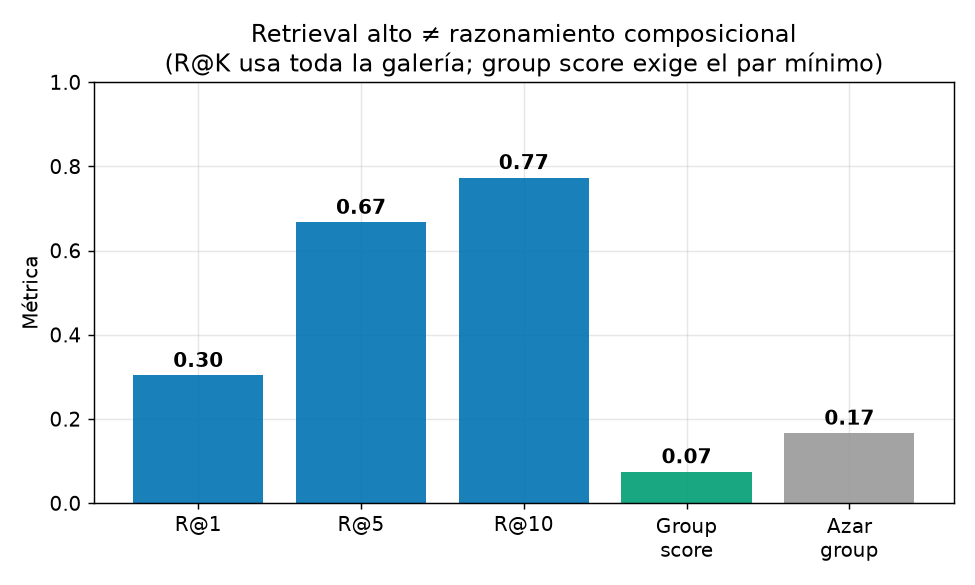
\includegraphics[height=0.42\textheight]{recall_vs_group.png}\end{center}
\end{frame}

% ----------------------------------------------------------- 3 min
\begin{frame}{Cómo lo obtuve ejecutando los cuadernos (3 min)}
  Reutilicé el \textbf{motor OpenCLIP del Cuaderno 10}: \texttt{create\_model\_and\_transforms},
  encode imagen/texto, similitud coseno.
  \begin{columns}
    \column{0.5\textwidth}
    \footnotesize
    \begin{enumerate}
      \item \texttt{winoground\_data.py}: real (HF, gated) + fallback curado.
      \item \texttt{openclip\_utils.py}: embeddings normalizados (C10).
      \item \texttt{winoground\_eval.py}: matriz $2\times2$ \texttt{sim[caption,imagen]} y los 3 scores.
      \item \texttt{02\_run\_winoground.py}: scores + IC bootstrap + by-tag + ceguera + R@K.
    \end{enumerate}
    \column{0.5\textwidth}
    \scriptsize
    \texttt{text=1 $\Leftrightarrow$ s(c0,i0)>s(c0,i1)\\ \hspace*{1.2em} y s(c1,i1)>s(c1,i0)}\\[2pt]
    \texttt{image=1 $\Leftrightarrow$ s(c0,i0)>s(c1,i0)\\ \hspace*{1.4em} y s(c1,i1)>s(c0,i1)}\\[2pt]
    \texttt{group = text AND image}
  \end{columns}
\end{frame}

% ----------------------------------------------------------- 3 min
\begin{frame}{Verificación en vivo: los tres scores (3 min)}
  \begin{center}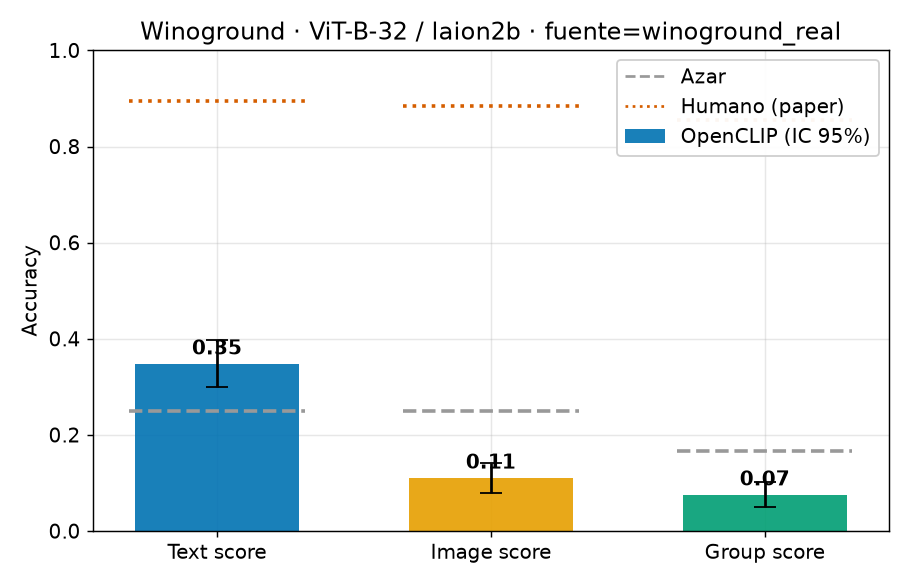
\includegraphics[height=0.78\textheight]{scores_vs_chance.png}\end{center}
\end{frame}

% ----------------------------------------------------------- 3 min
\begin{frame}{Mejora de código en vivo: ¿usa la imagen? y por tag (3 min)}
  \begin{columns}
    \column{0.5\textwidth}
    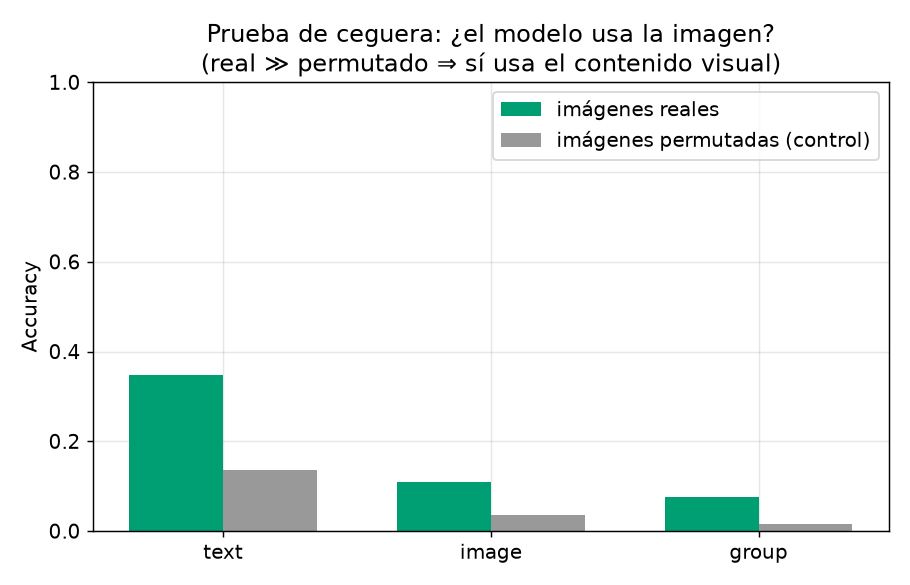
\includegraphics[width=\linewidth]{blindness.png}
    \column{0.5\textwidth}
    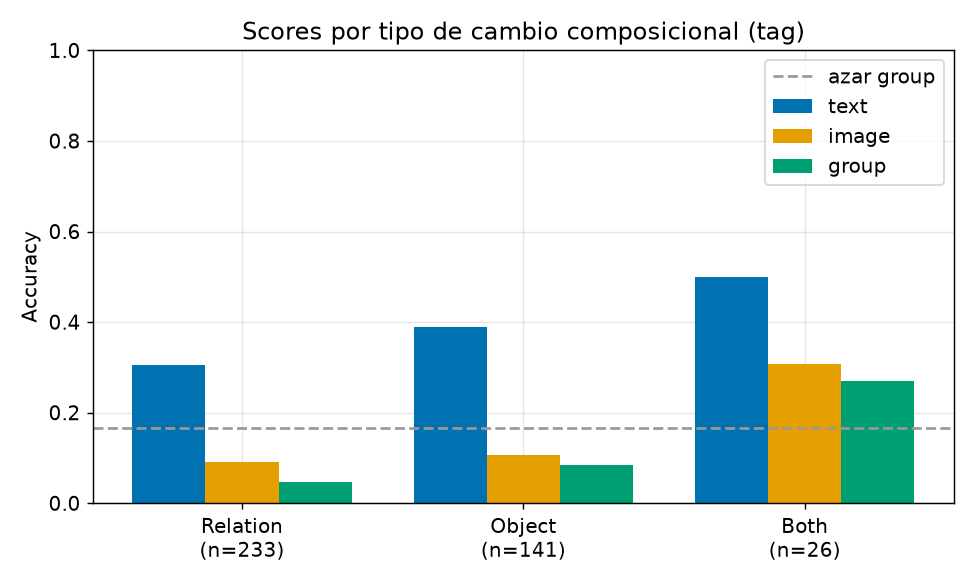
\includegraphics[width=\linewidth]{by_tag.png}
  \end{columns}
  \footnotesize Prueba de ceguera: real $\gg$ imágenes permutadas $\Rightarrow$ el modelo
  \emph{sí} usa la imagen. Los errores son de \textbf{binding/relación}, no de reconocimiento.
\end{frame}

% ----------------------------------------------------------- 2 min
\begin{frame}{Defensa crítica: limitaciones y mejora (2 min)}
  \begin{itemize}
    \item \textbf{Limitación:} el group score mezcla \emph{fallo composicional} con \emph{ítems ambiguos}
      (Diwan et al.); el set curado es un proxy controlado, no el benchmark oficial.
    \item \textbf{Métrica:} azar del group $=1/6$ (no $1/16$): text e image no son independientes.
    \item \textbf{Sesgo:} sensibilidad a empates y a la normalización de embeddings.
    \item \textbf{Mejora:} evaluar un \textbf{cross-encoder / fusión profunda (C5)} y re-ranking
      con interacción cruzada (C6); versionar embeddings (DVC) para reproducibilidad total.
  \end{itemize}
\end{frame}

\appendix
\begin{frame}{Backup: comparación de checkpoints}
  \begin{center}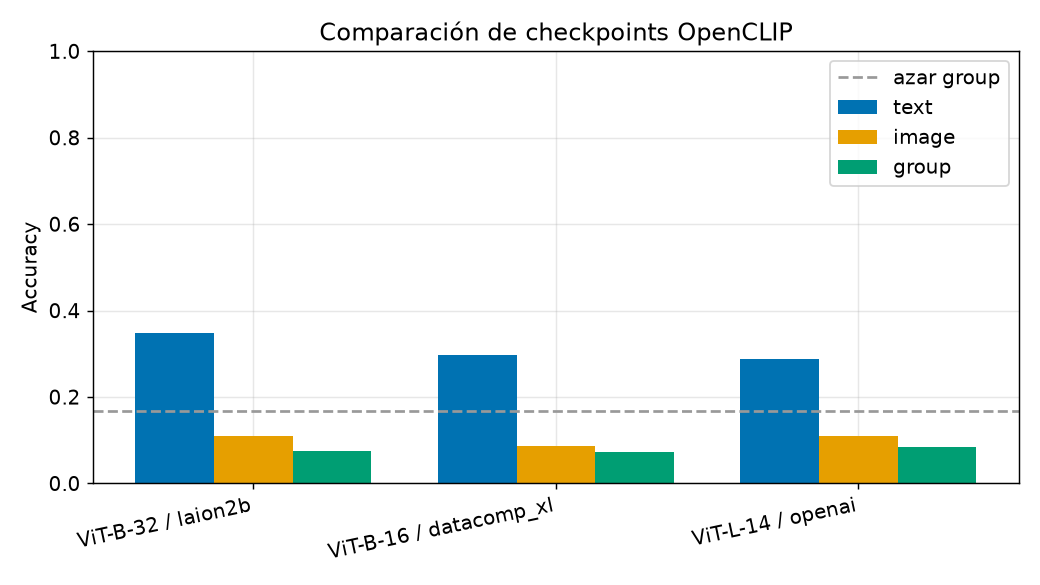
\includegraphics[height=0.7\textheight]{checkpoint_comparison.png}\end{center}
\end{frame}

\begin{frame}{Backup: casos de error}
  \begin{center}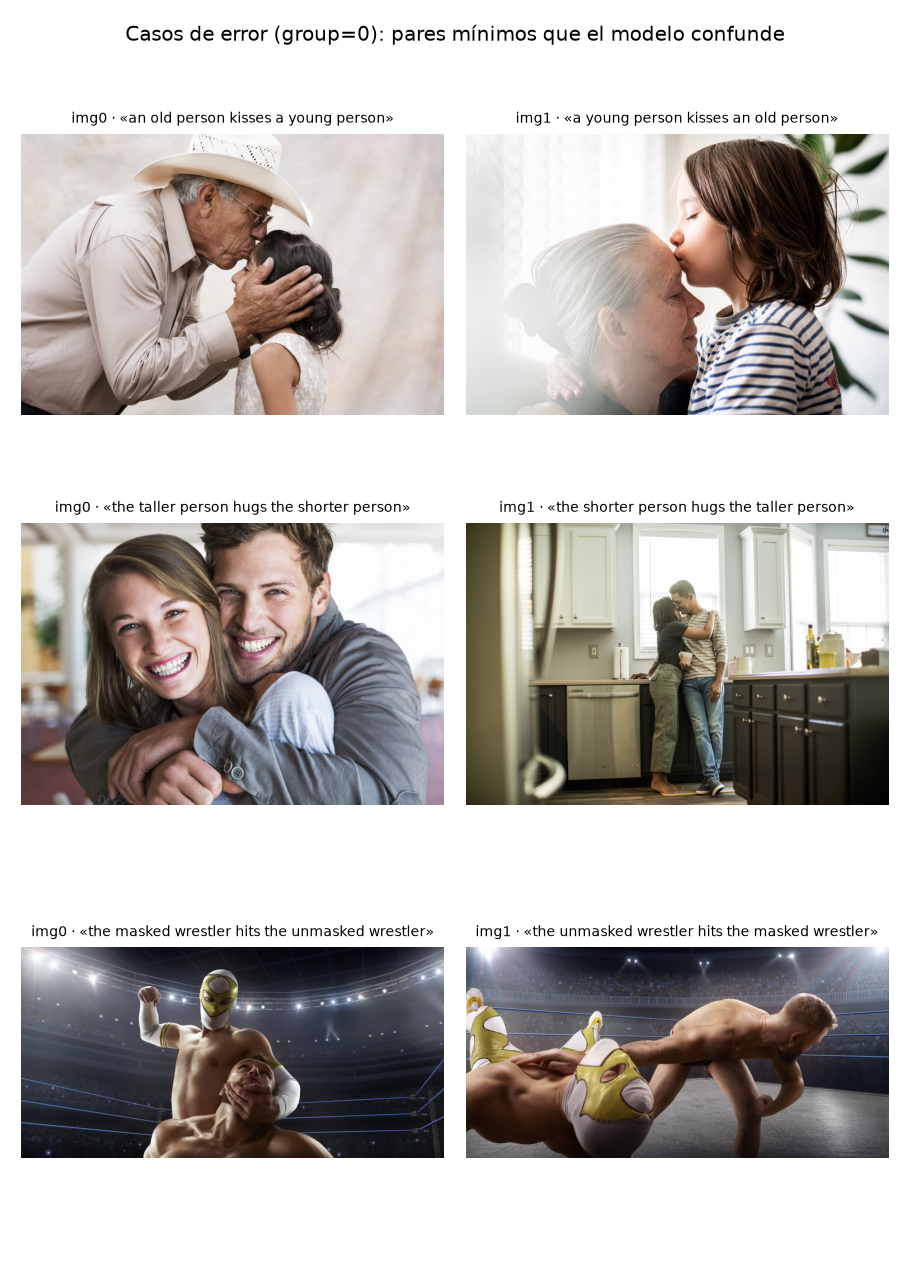
\includegraphics[height=0.72\textheight]{qualitative_examples.png}\end{center}
\end{frame}

\end{document}
